\chapter{Model Derivation for a Single Area Power System}
When looking at a single area power system, there are three main components that the literature has a tendency to focus on:
\begin{enumerate}
	\item \textbf{Governor:} used for controlling the angular velocity (and frequency) of the system;
	\item \textbf{Turbine:} this is the steam turbine which provides the mechanical torque to drive the generator; and
	\item \textbf{Generator load:} describes the electrical power that is produced and the electrical torque from connected loads. 
\end{enumerate}

%------------------------ S: Governor model
\section{Governor Model}
The most important part of a speed governor are the two large masses (the pair of balls) which spin around a central axis. These masses are mechanically coupled to the the turbine drive shaft, so their angular velocity is a function of the turbine speed. Elgerd's text provides a really great schematic representation of the governing system for a steam turbine, shown in Figure XXXX. This schematic is used to derive the plant model for the governor. 

\begin{figure}
	\centering
	\includegraphics[scale=0.5]{imagefile}
	\caption{text}
	\label{fig:A1_schematic_of_a_steam_governor}
\end{figure}

If we let $A$ on the in the schematic be moved downward a little bit, $\Delta y_A$, the turbine power output will change by a directly proportional amount. Letting $\Delta P_C$ be the power increase, this can be expressed as:
\begin{equation}
	\Delta y_A = k_C \Delta P_C
\end{equation}

An increase in $\Delta P_C$ will cause the pilot valve to move up, and high pressure oil will flow onto the top of the main piston forcing it downwards. As the steam valve opens, more steam will drive the turbine faster and causing the flyball governor to lower point $B$. Mathematically, the movement of $C$ can be expressed as the result of two separate inputs:
\begin{enumerate}
	\item Assuming that $\Delta y_A$ is small, using similar triangles, it can be written that:
	\begin{equation}
    	\Delta y_C = - \frac{l_2}{l_1} \Delta y_A
	\end{equation}
	\item Given a frequency increase $\Delta f$ point $B$ will move downward so, assuming $A$ is fixed, then using similar triangles it is clear that:
	\begin{equation}
		\Delta y_C = \frac{l_1 + l_2}{l_1} \Delta y_B
	\end{equation}
\end{enumerate}

Letting $k_1 = \frac{l_2}{l_1}$, $k_2 = \frac{l_1 + l_2}{l_1} k_2'$, and using equation XXXX, the total movement in point $C$ can be expressed as:
\begin{equation}
	\Delta y_C = - k_1 k_C \Delta P_C + k_2 \Delta f
\end{equation}

A similar analysis, considering movement of point $C$ and $E$, can be undertaken to mathematically express the movement of point $D$. The analysis also makes use of similar triangles and results in the expression:
\begin{equation}
	\Delta y_D = \frac{l_4}{l3 + l_4} \Delta y_C + \frac{l3}{l_3 + l_4} \Delta y_E
\end{equation}

Letting $k_3 = \frac{l_4}{l3 + l_4}$ and $k_4 = \frac{l3}{l_3 + l_4}$, this can be re-expressed as:
\begin{equation}
	\Delta y_D = k_3 \Delta y_C + k_4 \Delta y_E
\end{equation}

When there is some movement, $\Delta y_D$, of point $D$ the ports of the pilot valve will open and high pressure oil will plow onto the cylinder causing some movement $\Delta y_E$. If point $D$ moves up, high pressure oil will move point $E$ down, and conversely if point $D$ moves down, high pressure oil will move point $E$ upwards. To simplify the dynamics of this scenario, the following assumptions are made:
\begin{enumerate}
	\item Inertial reaction forces of the main piston and steam valve are negligible compared to the forces exerted on the piston by high pressure oil
	\item Due to the first assumption, the rate of oil admitted to to the cylinder is proportional to the port opening $\Delta y_D$.
\end{enumerate}

The volume of oil admitted to the cylinder is thus proportional to the time integral of $\Delta y_D$. Dividing the oil volume by the cross-sectional area of the piston:
\begin{equation}
	\Delta y_E = k_5 \int (- \Delta y_D) dt
\end{equation}

Taking the Laplace transform of equations XXXX, XXXX, and XXXX gives the following:


\begin{align}
	\Delta Y_C(s) &= -k_1 k_C \Delta P_C(s) + k_2 \Delta F(s) \\
	\Delta Y_D(s) &= k_3 \Delta Y_C(s) + k_4 \Delta Y_E(s) \\
	\Delta Y_E(s) &= - k_5 \frac{1}{s} \Delta Y_D(s)
\end{align}

Algebraically manipulating XXXX, XXXX, and XXXX eliminates $\Delta Y_C(s)$ and $\Delta Y_D(s)$ and results in the following equation:
\begin{equation}
	\Delta Y_E(s) = \frac{k_1 k_3 k_C \Delta P_C(s) - k_2 k_3 \Delta F(s)}{k_4 + \frac{s}{k_5}}
\end{equation}

Equation XXXX can be re-expressed as:
\begin{equation}
	\Delta Y_E(s) = \bigg[ \Delta P_C(s) - \frac{1}{R} \Delta F(s) \bigg] \times \bigg( \frac{K_{sg}}{1 + T_{sg}s} \bigg)
\end{equation}

where

\begin{align}
	R &= \frac{k_1 k_C}{k_2} \\
	K_{sg} &= \frac{k_1 k_3 k_C}{k_4} \\
	T_{sg} &= \frac{1}{T_{sg}} 
\end{align}

Equation XXXX is the model of the governor in the frequency domain. The parameter $R$ is referred to as the speed regulation of the governor; the parameter $K_{sg}$ is referred to as the gain of the speed governor; and the parameter $T_{sg}$ is referred to as the time constant of the speed governor.

The complete block diagram of governor model can be seen in Figure 2 below.

\begin{figure}
	\centering
	\input{}
	\caption{Block diagram of the steam governor model in the frequency domain}
	\label{}
\end{figure}

%------------------------ S: Turbine model
\section{Turbine Model}\label{app:turbine_model}
To develop a turbine model, consider a fossil-fuelled single reheat tandem-compound turbine. A basic configuration of components can be seen in Figure \ref{fig:A03_turbine_configuration}. The derivation and analysis that follows borrows heavily from Kundar \cite{Kundur1994}. Steam enters a high pressure (HP) section through the control valve and the inlet piping. Housing for the control valves is called the steam chest. The HP exhaust steam is passed through the re-heater. Reheat steam flows into the IP turbine section through the reheat intercept valve (IV) and the inlet piping. Crossover piping provides a path for the steam from IP section exhaust to the low pressure (LP) inlet.

\begin{figure}
	\centering
	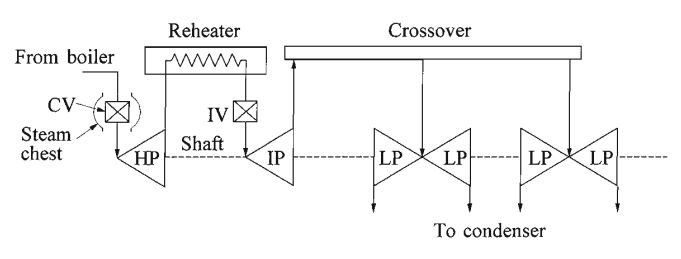
\includegraphics[scale=0.5]{A03_turbine_configuration}
	\caption[Reheat tandem-compound turbine configuration]{Configuration of a fossil-fuelled single reheat tandem-compound turbine \cite{Kundur1994}.}
	\label{fig:A03_turbine_configuration}
\end{figure}

Control valve position, $y_E$, modulates the steam flow through the turbine for load/frequency control during normal operation. The response of steam flow to a change in control valve position exhibits a time constant $T_{CH}$ due to the charging time of the steam chest and the inlet piping to the HP section. An intercept valve is normally used for rapid control of the turbine in the event of an overspeed; however, will not be considered in this analysis. The reheater holds a substantial amount of steam making the dynamics of this component slow enough to require its own time constant $T_{RH}$. Steam flowing into the LP sections experiences additional time constant $T_{CO}$ associated with the crossover piping. Figure 2 shows the block diagram representation of the tandem compound reheat turbine \cite{Kundur1994}.

\begin{figure}
	\centering
	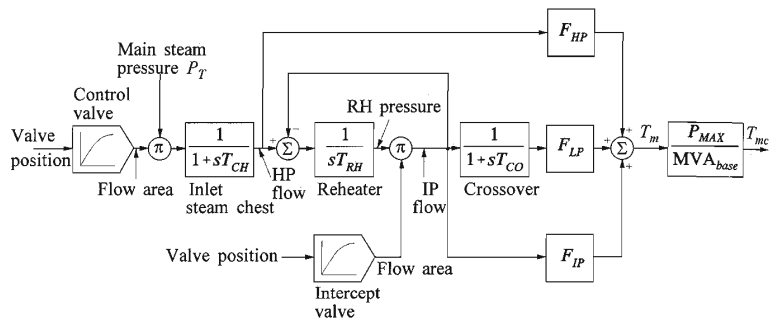
\includegraphics[scale=0.5]{A04_turbine_full_block_diagram}
	\caption[Tandem-compound reheat turbine model]{Block diagram of the tandem-compound reheat turbine \cite{Kundur1994}.}
	\label{fig:A04_turbine_full_block_diagram}
\end{figure}

To simplify the model shown in Figure \ref{fig:A04_turbine_full_block_diagram}, it is assumed that $T_{CO}$ is negligible in comparison to $T_{RH}$. Moreover, the remaining two time constants, $T_{CH}$ and $T_{RH}$, have been combined into a single time constant $T_t$. Hence, the power output of the turbine, $\Delta P_G(s)$, can be linked to the valve position, $\Delta Y_E(s)$, in the frequency domain with the following expression:
\begin{equation}
	\Delta F(s) = \bigg( \frac{K_t}{1 + T_t s} \bigg) \times P_G(s) \label{eq:A10}
\end{equation}

Equation \ref{eq:A10} is a simplified model of the turbine in the frequency domain. The parameter $K_t$ is referred to as the gain of the turbine; and the parameter $T_t$ is referred to as the time constant of the turbine. The block diagram showing this representation can be seen in Figure \ref{fig:A05_turbine_model}. 

\begin{figure}[h]
	\centering
	% Set up the standalone document class
\documentclass{standalone}

% Input the preamble (<3)
% Preamble document

% Import tikz package
\usepackage{tikz}

% Import tikz libraries
\usetikzlibrary{shapes, arrows}
\usetikzlibrary{positioning, calc}

%----------- Create a fancy summing block
\tikzset{add/.style n args={4}{
		minimum width=6mm,
		path picture={
			\draw[black] 
			(path picture bounding box.south east) -- (path picture bounding box.north west)
			(path picture bounding box.south west) -- (path picture bounding box.north east);
			\node at ($(path picture bounding box.south)+(0,0.13)$)     {\tiny #1};
			\node at ($(path picture bounding box.west)+(0.13,0)$)      {\tiny #2};
			\node at ($(path picture bounding box.north)+(0,-0.13)$)    {\tiny #3};
			\node at ($(path picture bounding box.east)+(-0.13,0)$)     {\tiny #4};
		}
	}
}

%----------- Block style 1
\tikzstyle{block1} = [draw, fill=blue!20, rectangle, 
minimum height=3em, minimum width=6em, node distance=2.5cm]

%----------- Block style 2
\tikzstyle{block2} = [draw, fill=blue!20, rectangle, 
minimum height=3em, minimum width=3em, node distance=2.5cm]

%----------- Sum style
\tikzstyle{sum} = [draw, fill=blue!20, circle, node distance=2cm]

%----------- Input style
\tikzstyle{input} = [coordinate, node distance=4cm]

%----------- Output style
\tikzstyle{output} = [coordinate, node distance=4cm]

%----------- Pin style
\tikzstyle{pinstyle} = [pin edge={to-,thin,black}]

\begin{document}

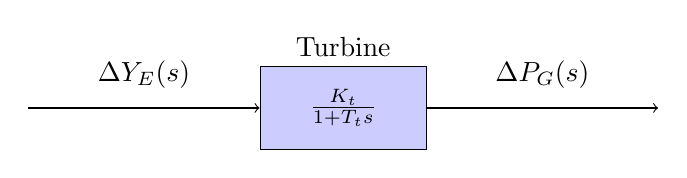
\begin{tikzpicture}

	% Draw the nodes first
	\node [input] (input) {};
	\node [block1, right of=input, node distance=4cm, label=above:{Turbine}] (turbine) {$\frac{K_{t}}{1 + T_{t}s}$};
	\node [output, right of=turbine] (output) {};
	
	% Connect the nodes
	\draw [->] (input) -- node [label=above:{$\Delta Y_E(s)$}] {} (turbine);
	\draw [->] (turbine) -- node [label=above:{$\Delta P_G(s)$}] {} (output);
	
\end{tikzpicture}

\end{document}
	\caption[Simplified turbine model]{Simplified block diagram of the tandem compound reheat turbine}
	\label{fig:A05_turbine_model}
\end{figure}

%------------------------ S: Generator-Load model
\section{Generator Load Model}
If the turbine output is in some steady state, and the power system experiences some perturbation, then let the incremental power from the turbine be $\Delta P_G$. Noting that the main perturbation experienced by a power system is the change in load demand, $\Delta P_L$, the incremental input to the generator-load system is given by $\Delta P_G - \Delta P_L$.

The increment in power input to the system is accounted for in two ways:
\begin{enumerate}
	
	\item Rate of increase of stored kinetic energy in the generator rotor. At scheduled frequency $f_0$, the stored energy is:
	\begin{equation}
		(W_{ke})_0 = H \times P_r,
	\end{equation}
	where $P_r$ is the kilowatt rating of the turbo-generator and $H$ is defined as it's inertial constant. Given that the kinetic energy is proportional to the square of the speed (frequency), the kinetic energy at a frequency of $f_0 + \Delta f$ can be written as:
	\begin{equation}
		W_{ke} = (W_{ke})_0 \bigg( \frac{f_0 + \Delta f}{f_0} \bigg)^2 \approx H P_r \bigg( 1 + \frac{2\Delta f}{f_0} \bigg)
	\end{equation}
	
	The rate of change of kinetic energy is therefore:
	\begin{equation}
		\frac{d}{dt}(W_{ke}) = \frac{2 H P_r}{f_0} \frac{d}{dt} (\Delta f) \label{eq:A11}
	\end{equation}
	
	\item Given that motors make up a reasonable percentage of the load demand it must be considered that the motor load changes as the frequency changes. The rate of change of load with respect to frequency, $\frac{\partial P_L}{\partial f}$, can be considered constant for small changes in frequency $\Delta f$ and can be expressed as:
	\begin{equation}
		\frac{\partial P_L}{\partial f} \Delta f = B \Delta f \label{eq:A12},
	\end{equation}
	where $B$ can be empirically determined, and is dependent on the proportion of motors that comprise the load demand. Note that is $B$ is positive, then the the load is predominantly comprised of motors.
\end{enumerate}

Using equations \ref{eq:A11} and \ref{eq:A12}, the power balance equation for the incremental input to the generator-load system can be written as:
\begin{equation}
	\Delta P_G - \Delta P_L = \frac{2 H P_r}{f_0} \frac{d}{dt} (\Delta f) + B \Delta f
\end{equation}

Dividing throughout by $P_r$ yields the following:
\begin{equation}
	\Delta P_G(pu) - \Delta P_L(pu) = \frac{2 H}{f_0} \frac{d}{dt} (\Delta f) + B(pu) \Delta f \label{eq:A13}
\end{equation}

Taking the Laplace transform of equation \ref{eq:A13} and rearranging, we get the following expression:
\begin{equation}
	\Delta F(s) = \frac{\Delta P_G(s) - \Delta P_L(s)}{B + \frac{2H}{f_0}s} \label{eq:A14}
\end{equation}

Equation \ref{eq:A14} can re-expressed as:
\begin{equation}
	\Delta F(s) = [\Delta P_G(s) - \Delta P_L(s)] \times \bigg( \frac{K_{gl}}{1 + T_{gl}} \bigg), \label{eq:A15}
\end{equation}
where
\begin{align}
K_{gl} &= \frac{1}{B} \\
T_{gl} &= \frac{2H}{B f_0}
\end{align}

Equation \ref{eq:A15} is the model of the generator-load in the frequency domain. The parameter $K_{gl}$ is referred to as the gain of the generator load; and the parameter $T_{gl}$ is referred to as the time constant of the generator load.

The complete block diagram of governor model can be seen in Figure XXXX below.

\begin{figure}[h]
	\centering
	% Set up the standalone document class
\documentclass{standalone}

% Input the preamble (<3)
% Preamble document

% Import tikz package
\usepackage{tikz}

% Import tikz libraries
\usetikzlibrary{shapes, arrows}
\usetikzlibrary{positioning, calc}

%----------- Create a fancy summing block
\tikzset{add/.style n args={4}{
		minimum width=6mm,
		path picture={
			\draw[black] 
			(path picture bounding box.south east) -- (path picture bounding box.north west)
			(path picture bounding box.south west) -- (path picture bounding box.north east);
			\node at ($(path picture bounding box.south)+(0,0.13)$)     {\tiny #1};
			\node at ($(path picture bounding box.west)+(0.13,0)$)      {\tiny #2};
			\node at ($(path picture bounding box.north)+(0,-0.13)$)    {\tiny #3};
			\node at ($(path picture bounding box.east)+(-0.13,0)$)     {\tiny #4};
		}
	}
}

%----------- Block style 1
\tikzstyle{block1} = [draw, fill=blue!20, rectangle, 
minimum height=3em, minimum width=6em, node distance=2.5cm]

%----------- Block style 2
\tikzstyle{block2} = [draw, fill=blue!20, rectangle, 
minimum height=3em, minimum width=3em, node distance=2.5cm]

%----------- Sum style
\tikzstyle{sum} = [draw, fill=blue!20, circle, node distance=2cm]

%----------- Input style
\tikzstyle{input} = [coordinate, node distance=4cm]

%----------- Output style
\tikzstyle{output} = [coordinate, node distance=4cm]

%----------- Pin style
\tikzstyle{pinstyle} = [pin edge={to-,thin,black}]

\begin{document}

\begin{tikzpicture}
	
	% Draw the nodes first
\end{tikzpicture}

\end{document}
	\caption[Generator-load model]{Block diagram of the generator load model in the frequency domain}
	\label{fig:A06_generator_load_model}
\end{figure}